\documentclass[aspectratio=169,11pt]{beamer}

\usepackage{advdate}
\usepackage{graphicx}

\definecolor{main}{HTML}{015697}
\definecolor{background}{HTML}{f8fbff}

\title{Introduction to CMake}
\author{Paolo Joseph Baioni}
\institute{Politecnico di Milano}
\AdvanceDate[1]
\date{\today}
\titlegraphic{}


\begin{document}
\begin{frame}[plain]{}
    \maketitle
\end{frame}

\section{Build systems}
\begin{frame}{Purposes}
    Build systems are a way to deploy software.
    \vfill
    They are used to
    \begin{enumerate}
        \item provide others a way to configure \textbf{your} own project;
        \item configure and install third-party software on your system.
    \end{enumerate}
    \vfill
    \textbf{Configure} means
    \begin{itemize}
        \item meet dependencies
        \item build
        \item test
    \end{itemize}
\end{frame}

\begin{frame}{Build systems generators available}
    \begin{itemize}
    \item \textbf{CMake}\footnote{\url{https://cmake.org/}}
    \begin{itemize}
    \item PRO: Easy to learn, great support for multiple IDEs, cross-platform
    \item CON: Does not perform automatic compilation test for met dependencies.
    \end{itemize}
    \item \textbf{GNU Autotools}\footnote{\url{https://www.gnu.org/software/automake/manual/}}
    \begin{itemize}
    \item PRO: Excellent support for legacy Unix platforms, large selection of existing modules.
    \item CON: Slow, hard to use correctly, painful to debug, poor support for non-Unix platforms.
    \end{itemize}
    \item \textbf{Meson}\footnote{\url{https://mesonbuild.com/}}, \textbf{Bazel}\footnote{\url{https://bazel.build/}}, \textbf{SCons}\footnote{\url{https://scons.org/}}, \dots
    \end{itemize}
\end{frame}

\begin{frame}{Leonardo Software Stack - 2024}
\begin{figure}
	\centering
	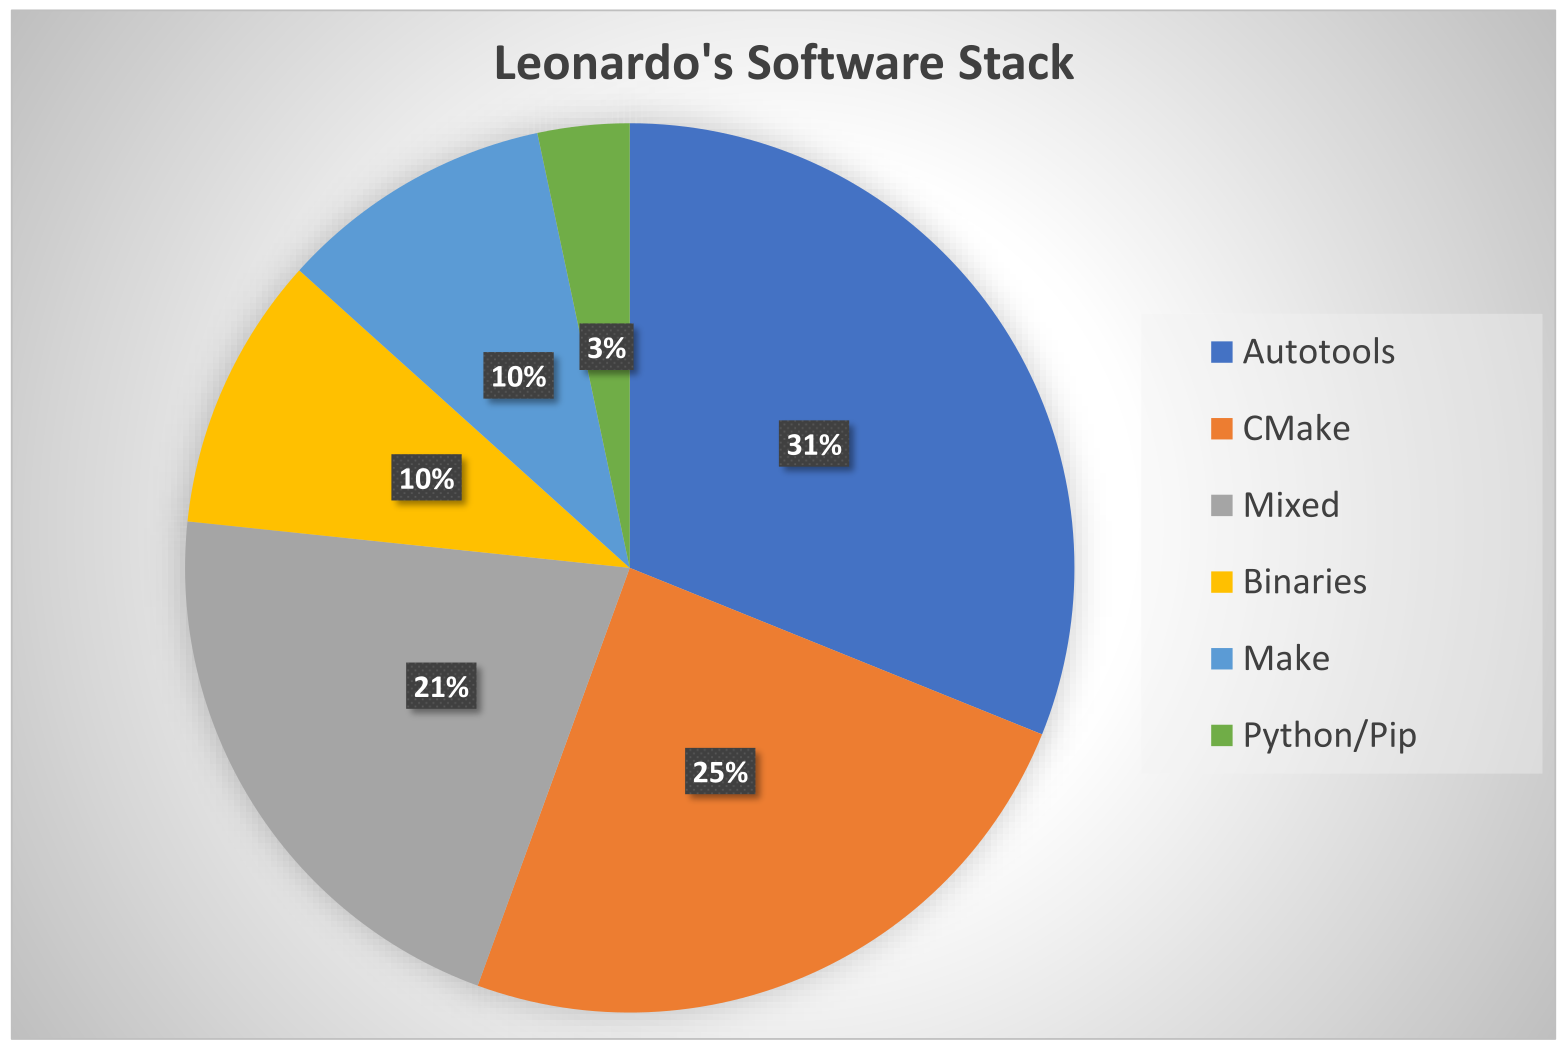
\includegraphics[width=0.7\linewidth]{img/cineca}
	\caption{Leonardo@CINECA, \href{https://www.top500.org/lists/top500/2024/11/}{\color{blue} top 9 hpc}}
	%\label{fig:cineca}
\end{figure}
\end{frame}

\begin{frame}{Build Systems Google Trends - 2024}
	\begin{figure}
		\centering
		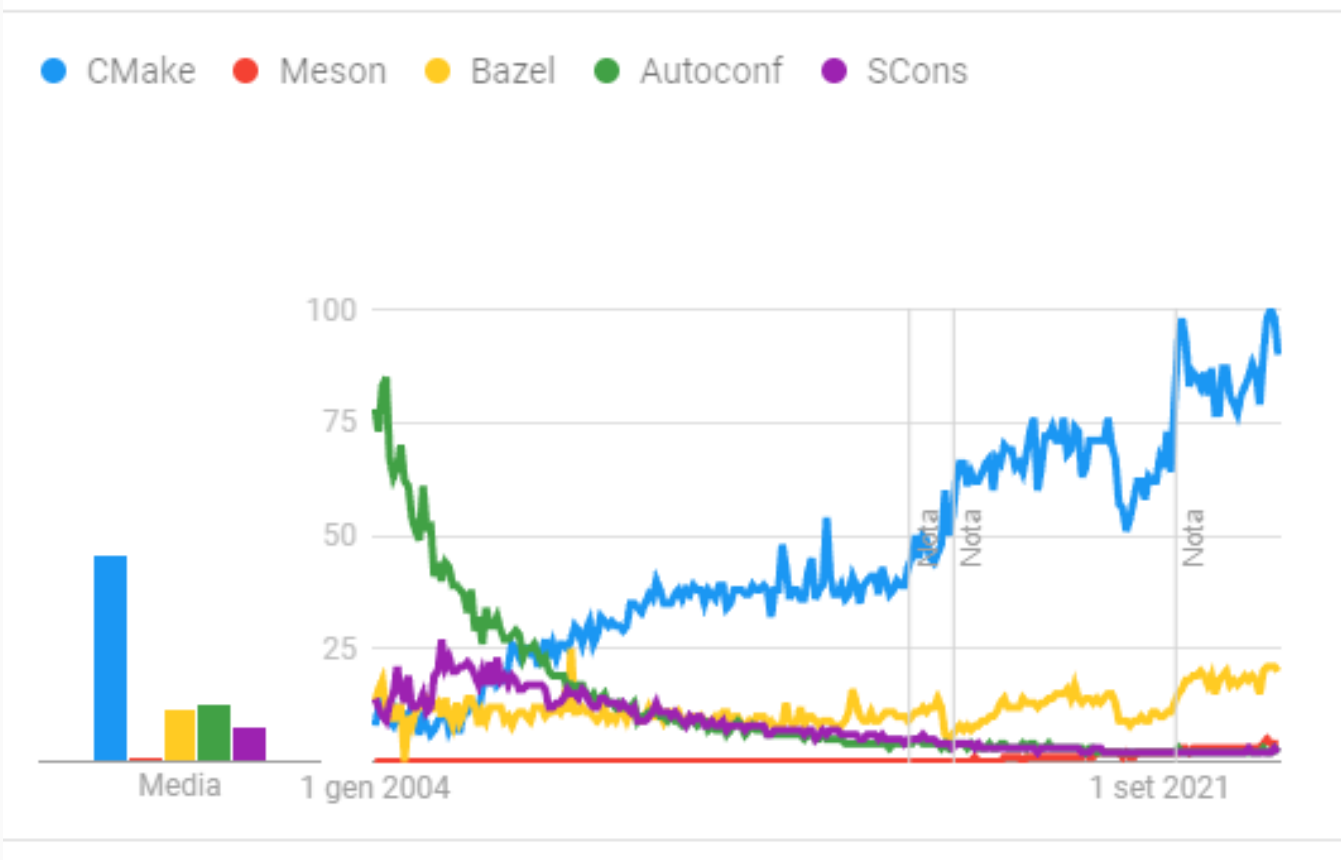
\includegraphics[width=0.7\linewidth]{img/google}
		\caption{Google Trends as of 2024}
		%\label{fig:google}
	\end{figure}
\end{frame}

\begin{frame}{Why CMake?}
\begin{itemize}
    \item More packages use CMake than any other system
    \item almost every IDE supports CMake (or vice-versa)
    \item really cross-platform, no better choices for Windows
    \item extensible, modular design
\end{itemize}
\vfill
\pause
Who else is using CMake?
\begin{itemize}
    \item Netflix
    \item HDF Group, ITK, VTK, Paraview (visualization tools)
    \item Armadillo, CGAL, LAPACK, Trilinos (linear algebra and algorithms)
    \item deal.II, Gmsh (FEM analysis)
    \item KDE, Qt, ReactOS (user interfaces and operating systems)
    \item \dots
\end{itemize}
\end{frame}

\begin{frame}{Resources}
\begin{itemize}
    \item Official documentation\\
    \url{https://cmake.org/cmake/help/latest/}
    \vfill
    \item Modern CMake\\
    \url{https://cliutils.gitlab.io/modern-cmake/}
    \vfill
    \item{It's time to do CMake right}\\
    \url{https://pabloariasal.github.io/2018/02/19/its-time-to-do-cmake-right/}
    \vfill
    \item Effective Modern CMake\\ \url{https://gist.github.com/mbinna/c61dbb39bca0e4fb7d1f73b0d66a4fd1}
    \vfill
    \item More Modern CMake\\ \url{https://www.youtube.com/watch?v=y7ndUhdQuU8&feature=youtu.be}
\end{itemize}
\end{frame}

\begin{frame}[fragile]{Let's try}
  Unload the \texttt{mk} module system (\texttt{module purge}), install dependencies then compile and install.\\
  \textbf{\{fmt\}} {\small (\url{https://github.com/fmtlib/fmt})}
  \begin{verbatim}
  cd /path/to/fmt/src/
  mkdir build && cd build
  cmake ..
  make -j<N>
  make test
  (sudo) make install
  \end{verbatim}
{ \color{gray} {
  \textbf{GNU Scientific Library} {\small (\url{https://www.gnu.org/software/gsl/})}
  \begin{verbatim}
  cd /path/to/gsl/src/
  ./configure --prefix=/opt/gsl --enable-shared --disable-static
  make -j<N>
  (sudo) make install
  \end{verbatim}
}}
\end{frame}

\section{CMake basics}
\begin{frame}[fragile]{CMake 101}
The root of a project using CMake must contain a \textbf{\texttt{CMakeLists.txt}} file.

\begin{verbatim}
cmake_minimum_required(VERSION 3.12)

# This is a comment.
project(MyProject VERSION 1.0
                  DESCRIPTION "A very nice project"
                  LANGUAGES CXX)
\end{verbatim}
Please use a CMake version more recent than your compiler (at least \(\geq 3.0\)).
\vfill
Command names are \textbf{case-insensitive}.
\end{frame}

\begin{frame}[fragile]{CMake 101}
Configure:
\begin{verbatim}
cmake -S /path/to/src/ -B build [options...]
# Or:
# mkdir build && cd build
# cmake /path/to/src/ [options...]
\end{verbatim}
Compile:
\begin{verbatim}
cd /path/to/build/
make -j<N>
\end{verbatim}
\vspace{-3mm}
\textbf{Remark:} this works iff the generator is Unix Makefiles; otherwise, or for portability\\ {\ttfamily cmake --build ./ build}\\
\vspace{3mm}
To print a list of variable values:
\begin{verbatim}
cd build
cmake /path/to/src/ -L
\end{verbatim}
\end{frame}

\begin{frame}[fragile]{Targets}
CMake is all about targets and properties. An executable is a target, a library is a target. Your application is built as a collection of targets depending on each other.

\begin{verbatim}
# Header files are optional.
add_executable(my_exec my_main.cpp my_header.h)

# Options are STATIC, SHARED (dynamic) or MODULE (plugins).
add_library(my_lib STATIC my_class.cpp my_class.h)
\end{verbatim}
\end{frame}

\begin{frame}[fragile]{Target properties}
Target can be associated various properties\footnote{\url{https://cmake.org/cmake/help/latest/manual/cmake-properties.7.html}}:
\begin{verbatim}
add_library(my_lib STATIC my_class.cpp my_class.h)
target_include_directories(my_lib PUBLIC include_dir)
# "PUBLIC" propagates the property to
# other targets depending on "my_lib".
target_link_libraries(my_lib PUBLIC another_lib)

add_executable(my_exec my_main.cpp my_header.h)
target_link_libraries(my_exec my_lib)
target_compile_features(my_exec cxx_std_20)
# Last command is equivalent to
# set_target_properties(my_exec PROPERTIES CXX_STANDARD 20)
\end{verbatim}
\end{frame}

\section{Interact with the outside world}
\begin{frame}[fragile]{Local variables}
\begin{verbatim}
set(LIB_NAME "my_lib")

# List items are space- or semicolon-separated.
set(SRCS "my_class.cpp;my_main.cpp")
set(INCLUDE_DIRS "include_one;include_two")

add_library(${LIB_NAME} STATIC ${SRCS} my_class.h)
target_include_directories(${LIB_NAME} PUBLIC ${INCLUDE_DIRS})

add_executable(my_exec my_main.cpp my_header.h)
target_link_libraries(my_exec ${LIB_NAME})
\end{verbatim}
\end{frame}

\begin{frame}[fragile]{Cache variables}
Cache variables are used to interact with the command line:
\begin{verbatim}
# "VALUE" is just the default value.
set(MY_CACHE_VARIABLE "VALUE" CACHE STRING "Description")

# Boolean specialization.
option(MY_OPTION "This is settable from the command line" OFF)
\end{verbatim}

Then:
\begin{verbatim}
cmake /path/to/src/ \
  -DMY_CACHE_VARIABLE="SOME_CUSTOM_VALUE" \
  -DMY_OPTION=OFF
\end{verbatim}
\end{frame}

\begin{frame}[fragile]{Useful variables}
\begin{description}
    \item[\texttt{CMAKE\_SOURCE\_DIR}]: top-level source directory
    \item[\texttt{CMAKE\_BINARY\_DIR}]: top-level build directory
\end{description}
\vspace{0.4cm}
If the project is organized in sub-folders:
\begin{description}
    \item[\texttt{CMAKE\_CURRENT\_SOURCE\_DIR}]: current source directory being processed
    \item[\texttt{CMAKE\_CURRENT\_BINARY\_DIR}]: current build directory
\end{description}
\vspace{0.2cm}
\begin{verbatim}
# Options are "Release", "Debug",
# "RelWithDebInfo", "MinSizeRel"
set(CMAKE_BUILD_TYPE Release)

set(CMAKE_CXX_COMPILER "/path/to/c++/compiler")
set(CMAKE_CXX_FLAGS "${CMAKE_CXX_FLAGS} -Wall")
set(CMAKE_LIBRARY_OUTPUT_DIRECTORY lib)
\end{verbatim}
\end{frame}

\begin{frame}[fragile]{Environment variables}
\begin{verbatim}
# Read.
message("PATH is set to: $ENV{PATH}")

# Write.
set(ENV{variable_name} value)
\end{verbatim}

(although it is generally a good idea to avoid them).
\end{frame}

\begin{frame}[fragile]{Control flow}
\begin{verbatim}
if("${variable}")
    # True if variable is not false-like
else()
    # Note that undefined variables would be `""` thus false
endif()
\end{verbatim}
\vfill
The following operators can be used.
\vfill
Unary: \texttt{NOT}, \texttt{TARGET}, \texttt{EXISTS} (file), \texttt{DEFINED}, etc.\\
Binary: \texttt{STREQUAL}, \texttt{AND}, \texttt{OR}, \texttt{MATCHES} (regular expression), \dots
\vfill
Parentheses can be used to group.
\end{frame}

\begin{frame}[fragile]{Print messages and debug}
Content of variables is printed with
\begin{verbatim}
message("MY_VAR is: ${MY_VAR}")
\end{verbatim}
\vfill
Error messages can be printed with
\begin{verbatim}
message(FATAL_ERROR "MY_VAR has wrong value: ${MY_VAR}")
\end{verbatim}
\vfill
Commands being executed are printed with
\begin{verbatim}
cmake /path/to/src/ -B build --trace-source=CMakeLists.txt
make VERBOSE=1
\end{verbatim}
\end{frame}

\section{Advanced CMake}
\begin{frame}[fragile]{Looking for third-party libraries}
CMake looks for \textbf{module files} \texttt{FindPackage.cmake} in the directories specified in \texttt{CMAKE\_PREFIX\_PATH}.
\vfill
\begin{verbatim}
set(CMAKE_PREFIX_PATH "${CMAKE_PREFIX_PATH} /path/to/module/")

# Specify "REQUIRED" if library is mandatory.
find_package(Boost 1.50 COMPONENTS filesystem graph)
\end{verbatim}
\vfill
If the library is not located in a system folder, often a hint can be provided:
\begin{verbatim}
cmake /path/to/src/ -DBOOST_ROOT=/path/to/boost
\end{verbatim}
\end{frame}

\begin{frame}[fragile]{Using third-party libraries}
Once the library is found, proper variables are populated.
\begin{verbatim}
if(${Boost_FOUND})
    target_include_directories(my_lib PUBLIC
                               ${Boost_INCLUDE_DIRS})
    
    target_link_directories(my_lib PUBLIC
                            ${Boost_LIBRARY_DIRS})
    # Old CMake versions:
    # link_directories(${Boost_LIBRARY_DIRS})
    
    target_link_libraries(my_lib ${Boost_LIBRARIES})
endif()
\end{verbatim}
\end{frame}

\begin{frame}[fragile]{Branch selection}
Useful for switching among different implementations or version of any third-party library.
\vfill
\texttt{my\_main.cpp}:
\begin{verbatim}
#ifdef USE_ARRAY
    std::array<double, 100> my_array;
#else
    std::vector<double> my_array;
#endif
\end{verbatim}

How to select the correct branch?
\end{frame}

\begin{frame}[fragile]{Pre-processor flags}
\texttt{CMakeLists.txt}:
\begin{verbatim}
target_compile_definitions(my_exec PRIVATE USE_ARRAY=1)
\end{verbatim}
Or let user set the desired flag:
\begin{verbatim}
option(WITH_ARRAY "Use std::array instead of std::vector" ON)

if(WITH_ARRAY)
    target_compile_definitions(my_exec PRIVATE USE_ARRAY=1)
endif()
\end{verbatim}
\end{frame}

\begin{frame}[fragile]{Modify files depending on variables}
\texttt{print\_version.hpp.in}:
\begin{verbatim}
void print_version() {
  std::cout << "Version number: " << @MY_PROJECT_VERSION@
            << std::endl;
}
\end{verbatim}
\texttt{CMakeLists.txt}:
\begin{verbatim}
set(MY_PROJECT_VERSION 1.2.0)

configure_file(
  "${CMAKE_CURRENT_SOURCE_DIR}/print_version.hpp.in"
  "${CMAKE_CURRENT_BINARY_DIR}/print_version.hpp")
\end{verbatim}
See also: \texttt{\#cmakedefine}.
\end{frame}

\begin{frame}[fragile]{Compilation test}
CMake can try to compile a source and save the exit status in a local variable.
\begin{verbatim}
try_compile(
    HAVE_ZIP
    "${CMAKE_BINARY_DIR}/temp"
    "${CMAKE_SOURCE_DIR}/tests/test_zip.cpp"
    LINK_LIBRARIES ${ZIP_LIBRARY}
    CMAKE_FLAGS
        "-DINCLUDE_DIRECTORIES=${ZIP_INCLUDE_PATH}"
        "-DLINK_DIRECTORIES=${ZIP_LIB_PATH}")

# See also.
try_run(...)
\end{verbatim}
\end{frame}

\begin{frame}[fragile]{Execution test}
CMake can run specific executables and check their exit status to determine (un)successful runs.
\begin{verbatim}
include(CTest)
enable_testing()
add_test(NAME MyTest COMMAND my_test_executable)
\end{verbatim}
\end{frame}

\begin{frame}[fragile]{Organize a large project}
\begin{verbatim}
# Set the minimum required version of CMake
cmake_minimum_required(VERSION 3.12)

# Set the project name and version
project(ScientificProject VERSION 1.0 LANGUAGES CXX)

# Define the source, include and test directories
set(SOURCE_DIR ${CMAKE_SOURCE_DIR}/src)
set(INCLUDE_DIR ${CMAKE_SOURCE_DIR}/include)
set(TEST_DIR ${CMAKE_SOURCE_DIR}/tests)

# Include directories
include_directories(${INCLUDE_DIR})

# Find and include external dependencies (e.g., Boost, Eigen)
find_package(...)
\end{verbatim}
\end{frame}


\section{Tip: how to organize a large project}
\begin{frame}[fragile]
\small
\begin{minipage}[t]{.5\linewidth}
\begin{verbatim}
ScientificProject/
├── CMakeLists.txt
├── README.md
├── LICENSE
├── .gitignore
├── cmake/
│   └── FindSomeLib.cmake
├── include/
│   ├── module1/
│   │   ├── module1.h
│   │   └── module1_utils.h
│   └── module2/
│       ├── module2.h
│       └── module2_utils.h
├── src/
│   ├── CMakeLists.txt
│   ├── main.cpp
│   ├── module1/
│   │   ├── CMakeLists.txt
\end{verbatim}
\end{minipage}%
\begin{minipage}[t]{.5\linewidth}
\begin{verbatim}
	│   │   ├── module1.cpp
	│   │   └── module1_utils.cpp
│   └── module2/
│       ├── CMakeLists.txt
│       ├── module2.cpp
│       └── module2_utils.cpp
├── tests/
│   ├── CMakeLists.txt
│   ├── test_module1.cpp
│   ├── test_module2.cpp
│   └── test_utils.cpp
├── data/
│   ├── dataset1.csv
│   └── dataset2.csv
├── docs/
│   ├── API.md
│   └── UserGuide.md
└── scripts/
│   ├── do_something.sh
│   ├── another_script.py
\end{verbatim}
\end{minipage}
\end{frame}

\end{document}
